\documentclass{article}
\usepackage[utf8]{inputenc}

\usepackage{natbib}
\usepackage{graphicx}
\usepackage{fancyhdr}

\pagestyle{fancy}
\fancyhf{}
\fancyfoot[L]{Unless otherwise specififed, all content is the author's summary of "Goodfellow, Ian, Yoshua Bengio, and Aaron Courville. Deep learning. MIT press, 2016."}

\title{Deep Learning Textbook - Notes}
\author{yusuf.roohani }
\date{August 2017}

\begin{document}
\maketitle
\section{Probability}

\subsection{Distributions}

\begin{itemize}
    \item Probability mass functions:\\
    State of the random variable $\mapsto$ Probability of the variable taking on that state
    
    \item Joint probability functions:
    Probability distribution over multiple variables
    
    \item 
    For any probability mass function:
    \begin{itemize}
    \item Domain of P should be all possible states of x
    \item $\forall$ $x \in$ x, $ 0 \leq P(x) < 1$
    \item $\sum_{x \in \textrm{x}} P(x) = 1$
    \end{itemize}
\end{itemize}

\section{Neural networks}

\begin{itemize}
    \item \textbf{Softmax} The softmax function is normally used to highlight the largest values and suppress values which are significantly below the maximum value
\end{itemize}

\section{Regularization}
Central problem in machine elarning is to perform well not only on training data, but also on new inputs. \textbf{Regularization refers to any modification to a learning algorithm that is intended to reduce its generalization error but not its training error}

In deep learning, a common approach is to regularize estimators: this is done by trading increased bias for reduced variance. Try to improve effectiveness by making a profitable trade. Models are generally in three regimes
\begin{itemize}
    \item \textbf{Underfitting}: Exclude the true data-generating process
    \item Matched the true data generating process
    \item \textbf{Overfitting}: Include the process but also many other possible generating processes
\end{itemize}
The goal of regularization is to take a model from the third regime to the second regime. What we generally find is that the best fitting model is a large model that has been regularized appropriately.

\subsection{Parameter Norm Penalties}

Limit the capacity of models by adding a paramter norm penalty $\Omega(\theta)$ to the objective function $J$. 
$$ \tilde{J}(\theta; X, y) = J( \theta; X, y) + \alpha\Omega(\theta) $$

where $ \alpha \in [0, \infty) $ is a hyperparamter that weighs the relative contribution of the norm penalty term, $\Omega$, relative to the standard objective function J.

So the training algorithm will decrease both $J$ and some measure of the size of some subset of the parameters $ \theta$.

Generally, for neural networks, we \textbf{only penalize the weights of the affine transformation and not the biases}. Bias controls only a single variable whereas the weights determine how two variables interact. Regularizing bias can induce significant underfitting.

\begin{itemize}
    \item \textbf{$L^2$ Regularization} Also known as the weight decay, this regularization strategy drives the weights closer to the origin by adding a term $ \Omega(\theta) = \frac{1}{2} || w ||^2_2$
    
    So, the objective function can be written as:
    $$ \tilde{J}(w; X, y) = J(w; X, y) + \frac{\alpha}{2}w^Tw $$
    
    And the update step after simplification becomes:
    $$ w \leftarrow (1 - \epsilon\alpha)w - \epsilon \nabla_wJ(w; X,y) $$
    
    Clearly, there is a multiplicative shrinking of the weight vector by a constant factor on each step.
    
    ----
    
    Only directins along which the paramters contribute significantly to reducing the objective function are preserved relatively intact. In others, a small Eigen value of the Hessian tells us that movement in that direction will not significantly increase the gradient.
    
    In the specific case of linear regression, this equation is simplified to:
    $$ w = (X^TX + \alpha I) ^{-1} X^T y $$
    
    Since the diagonal entries of $ (X^TX + \alpha I)$ correspond to the variance of each input feature, we see that $L^2$ regularization causes $X$ to appear as though it has higher variance. The algorithm thus shrinks weights on features whose covariance with the output target is low compared with the added variance .
    
    \item{$L^1$ Regularization} - Here we add the absolute value of the individual parameters to $J$
    
    $$ \Omega(\theta) = ||w||_1 = \sum_i|w_i| $$
    
    
    
\end{itemize}

Reinforcement Learning

\begin{figure}[h!]
\centering
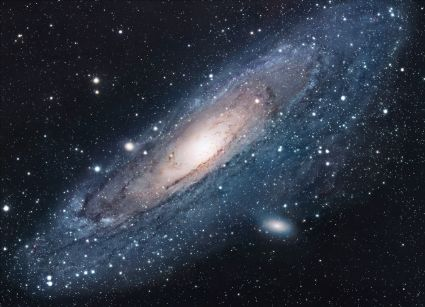
\includegraphics[scale=1.7]{universe.jpg}
\caption{The Universe}
\label{fig:univerise}
\end{figure}

\section{Conclusion}
``I always thought something was fundamentally wrong with the universe'' \citep{adams1995hitchhiker}

\bibliographystyle{plain}
\bibliography{references}

\end{document}
